
Every experimental science suffer from the same problem, evaluation of the data already collected. Even the simple idea of collecting data can become a painful task, because the measurement process may introduce errors, or cause distortion in the data. But we are now concerned in analyzing the data already collected.

A measure has itself noise, that may have come from the processes running in background, the operating system calls, interruptions, memory allocation, and other sources of noise, including the measurement process itself. Hence, one of the most important tasks is to have a good understanding of the noise that our system has \cite{Kalibera2013}.

This is an important issue, because we know that there is noise, that we cannot avoid it, but we can cope with it. In \cite{Kalibera2013}, we may see that the majority of the experimental studies lack a rigorous statistical methodology, which their work tries to fill in. In our case, we also are worried with such issues and we also proposed another way to evaluate and collect data, the \CP\ methodology cite{BerubePhD}. Therefore we chose to use the initial steps proposed in \cite{Kalibera2013}, to further characterize the noise in our experimental data.

To show the gaussian variation in the data we collect, \refFigure{fig:gauss} depicts a scatter plot of $1000$ sequential runs of the program \bzip, after being compiled using the \funcname{Static} inliner (\llvm) whose input was {\tt ebooks}. The figure shows a gaussian noise around the median plus a few outliers, generated by the operating system regular use. These outliers are filtered off from the data we are using. They are easily discarded because they have much more variance (more than one deviation from the median).

\begin{figure}
  \centering
  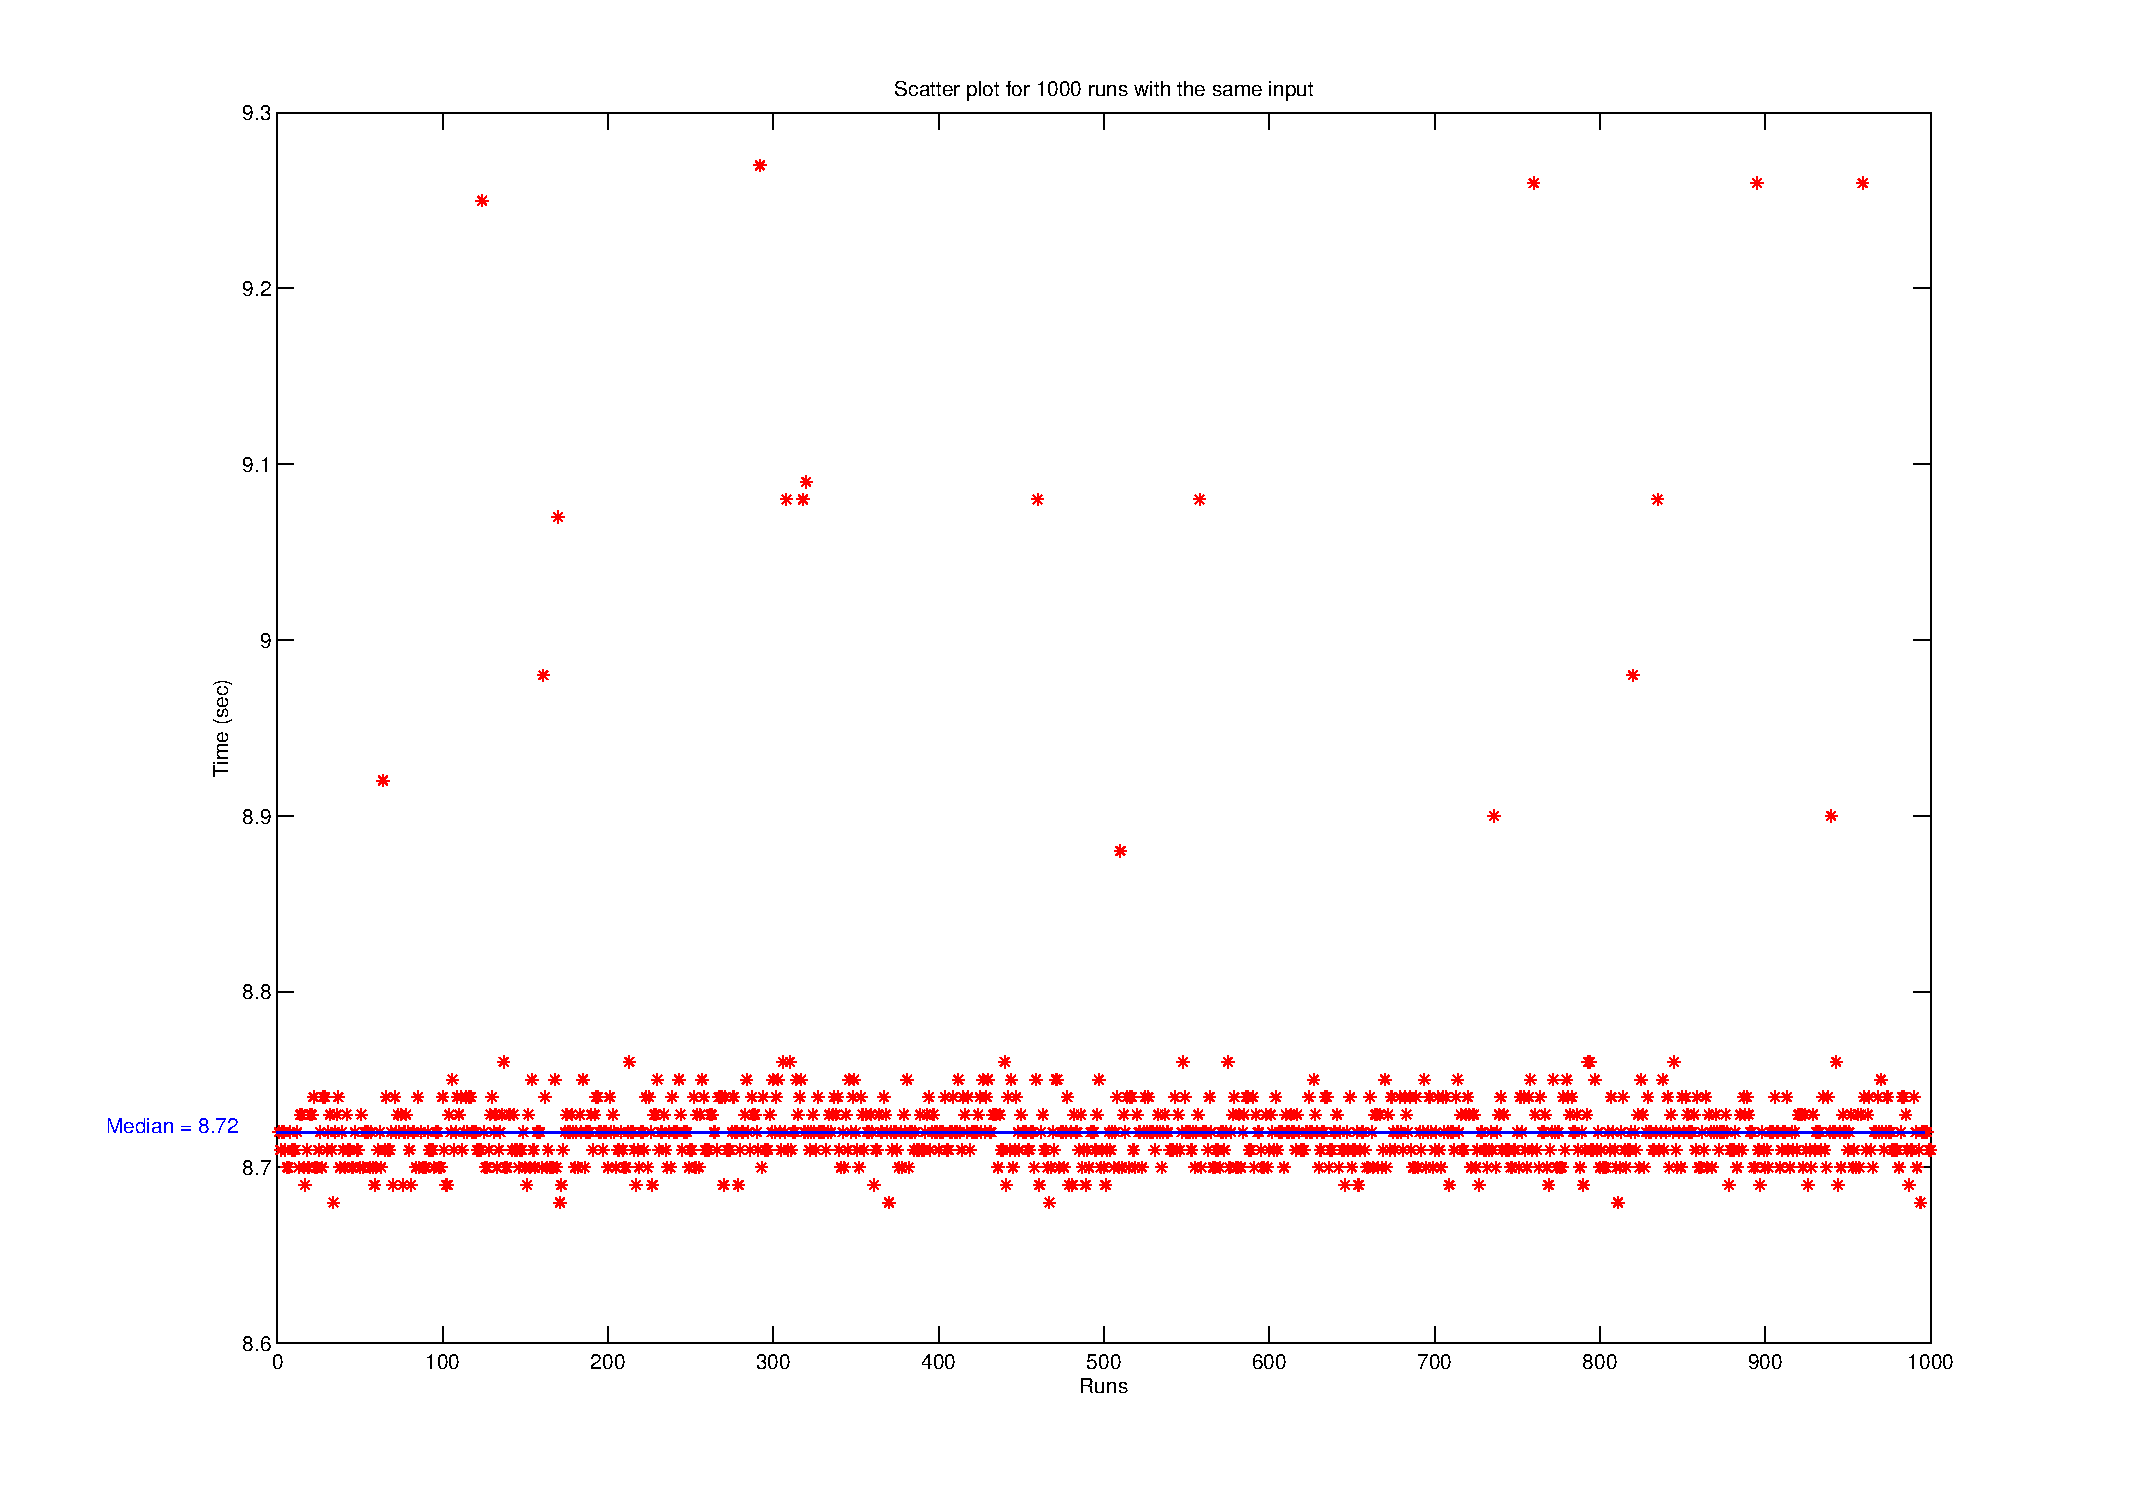
\includegraphics[width=1.00\linewidth]{Figures/nt1000}
  \caption{Running $1000$ times the same program with the same input data}
  \label{fig:gauss}
\end{figure}

We ran three independent experiments, the first is the $10$-times experiment, then $100$-times and, after that, $1000$-times, because we needed to confirm that there is no difference on their means, and also that we can discard the outliers. To make sure that we have robust measures, we ran some simple statistics to know the mean, the median, the standard-deviation from the mean (std-mean), and the standard-deviation from the median (std-median), shown in \refTable{tab:robustTest}. We also ran t-tests on each sample pairs to verify if their means were the same, the results for the t-tests are shown in \refTable{tab:ttest} below.

\begin{table}
  \centering
  \begin{tiny}
  
\begin{tabular}{lllll}

{\bf Length} & {\bf Mean} & {\bf Median} & 
  {\bf StD Mean} & {\bf StD Median} \\ \hline

10   & 8.7160 & 8.7150 & 0.0100 & 0.0050 \\
100  & 8.7328 & 8.7200 & 0.0187 & 0.0100 \\
1000 & 8.7248 & 8.7200 & 0.0197 & 0.0100 \\

\hline
\end{tabular}

  \end{tiny}
  \caption{Simple statistics on the experiment}
  \label{tab:robustTest}
\end{table}

The t-tests in \refTable{tab:ttest} show that the null hypothesis cannot be discarded, as the value $0$ in each line of the \emph{t-test} column confirms. The \emph{p-values} illustrate the confidence in the hypothesis, in this case, that the means are different.

\begin{table}
  \centering
  \begin{tiny}
  
\begin{tabular}{lllll}

{\bf Runs} & {\bf Reject $H_0$} & {\bf p-value}  \\ \hline

(10-100) & No & 0.3424  \\
(10-1000) & No & 0.6025 \\
(100-1000) & No & 0.1528 \\

\hline
\end{tabular}

  \end{tiny}
  \caption{t-tests applied pairwise to the $10$, $100$, and $1000$ runs}
  \label{tab:ttest}
\end{table}

Our experiments have also shown that the variance when running the same data just three times in a row is not quite different from the one running $100$ times. When we consider each `input-run' a $3$-consecutive run -- which means we ran $300$ times the same experiment --, and we consider a `full-run' as running a $3$-consecutive run to each input. We ran $100$ `full-runs' in this experiment, and we put some extra noise at its end.

What this means is that even though the effect of the noise can mask the correct values, we can treat them in order to assure robustness. This is the way we employed to empirically verify the soundness of the \CP\ methodology. As \refFigure{fig:CProbust} below shows, the deviation from the mean is not large, but here is a subtle knob increasing the running time of the all programs in the experiment by its end. It was caused by the execution of another system at the same time competing for the same resources. In (\refFigure{CP:ebooks}) we depicted in the $y$-axis the running time for each program at each 3-consecutive run, which are depicted on the $x$-axis. It can be also visualised in the histogram (\refFigure{CP:hist}). These figures show the $3$-consecutive run for the input data {\tt ebooks}, where in the $x$-axis we depicted the running time for the program and on the $y$-axis we depicted the number of runs at each bin.

\begin{figure}
  \centering
  \begin{minipage}[t]{\linewidth}
    \subfigure[$100$-time runs of the $3$-consecutive execution of input {\tt ebooks} for program \bzip] {
      \begin{minipage}[b]{0.75\textwidth}
        \centering
        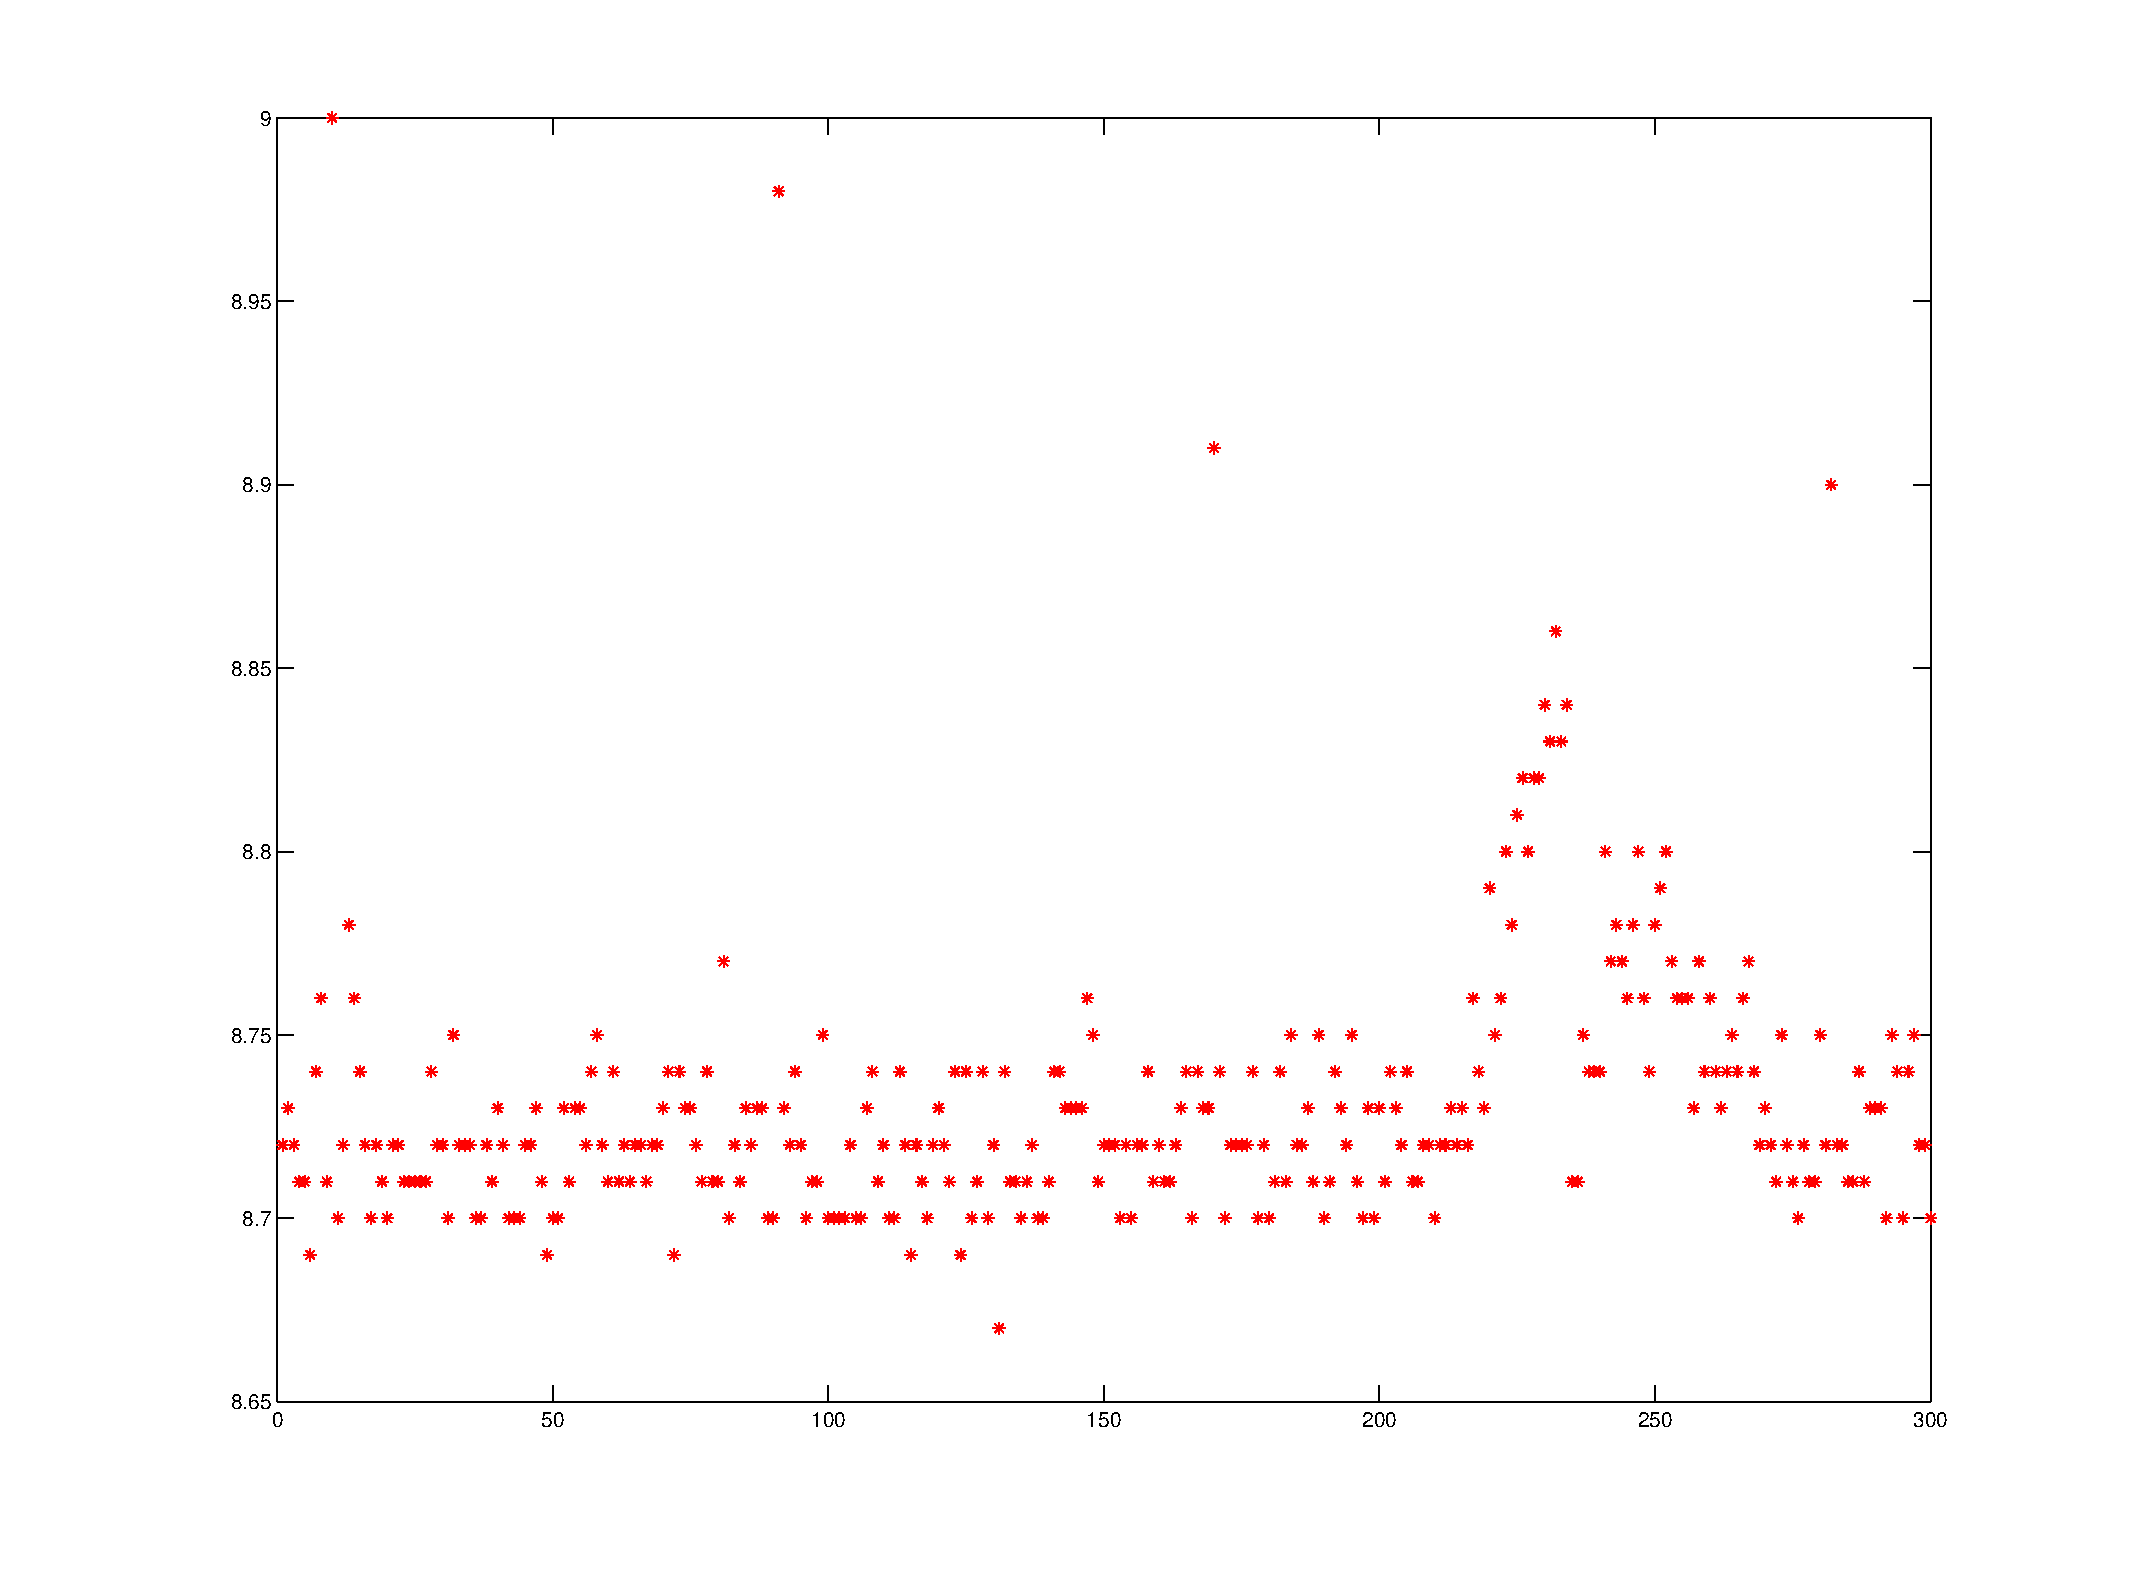
\includegraphics[height=12em]{Figures/ebooks300}
      \end{minipage}
      \label{CP:ebooks}
    }
    \vspace{1em}
    \hrule
    \vspace{1em}
    \subfigure[Histogram for the {\tt auriel} input] {
      \begin{minipage}[b]{0.75\textwidth}
        \centering
        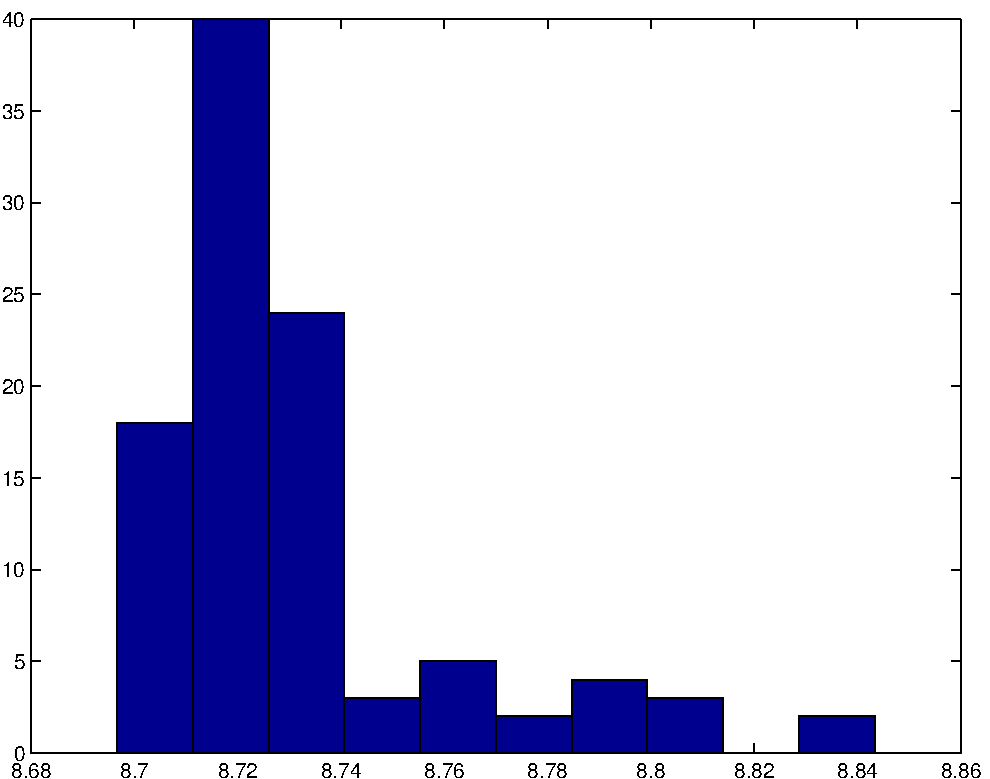
\includegraphics[height=12em]{Figures/ebooks}
      \end{minipage}
      \label{CP:hist}
    }
  \end{minipage}
  \caption{$100$-times running $3$-consecutive experiment}
  \label{fig:CProbust}
\end{figure}

The figures \refFigure{fig:CProbust} and \refFigure{fig:gauss} show that collecting data from single execution can produce erroneous results, even using machines with no other running program, we still have some noise due to operating system activities, interruptions, etc. And also that a simple inclusion of a simple job during the running cycle can perturb the execution time, as can be observed by the knob in \refFigure{fig:CProbust}.

The robustness is achieved when we can statistically assure that the variance on the data is not large.
The data used in the experiment are shown in \refTable{tab:simStats}, and the deviations from the mean (and median) to each $3$-consecutive run are summarized as the average, minimum, and maximum values, all found on the $300$-times experiment.

\begin{table}
  \centering
  \begin{tiny}
  
\begin{tabular}{lllll}

{\bf Run} & {\bf Mean} & {\bf Median} & 
  {\bf StD Mean} & {\bf StD Median} \\ \hline

1 & 8.7233 & 8.72 & 0.0044   \\
2 & 8.71 & 8.71 & 0.0067 & 0.01   \\
3 & 8.72 & 8.73 & 0.02 & 0.01   \\
4 & 8.7067 & 8.7 & 0.0089 & 0.00   \\
5 & 8.71 & 8.71 & 0.0067 & 0.01   \\
6 & 8.7933 & 8.74 & 0.0778 & 0.01   \\
7 & 8.73 & 8.73 & 0.0067 & 0.01   \\
8 & 8.7233 & 8.71 & 0.0178 & 0.00   \\
9 & 8.73 & 8.73 & 0.0067 & 0.01   \\
10 & 8.7033 & 8.71 & 0.0089 & 0.00   \\
\\
33 & 8.71 & 8.71 & 0.0067 & 0.01   \\
34 & 8.7267 & 8.73 & 0.0044 & 0.00   \\
35 & 8.71 & 8.7 & 0.0133 & 0.00   \\
36 & 8.81 & 8.73 & 0.1133 & 0.01   \\
37 & 8.72 & 8.72 & 0.0133 & 0.02   \\
\\
70 & 8.72 & 8.71 & 0.0133 & 0.00   \\
71 & 8.7133 & 8.72 & 0.0089 & 0.00   \\
72 & 8.7233 & 8.72 & 0.0044 & 0.00   \\
73 & 8.7233 & 8.72 & 0.0044 & 0.00   \\
74 & 8.743333 & 8.74 & 0.0111 & 0.01   \\
75 & 8.7667 & 8.76 & 0.0156 & 0.01   \\
76 & 8.7967 & 8.8 & 0.0111 & 0.01   \\
77 & 8.8133 & 8.82 & 0.0089 & 0.00   \\
78 & 8.83 & 8.83 & 0.0067 & 0.01   \\
79 & 8.8433 & 8.84 & 0.0111 & 0.01   \\
80 & 8.74 & 8.74 & 0 & 0.00   \\
81 & 8.7833 & 8.78 & 0.0111 & 0.01   \\
82 & 8.77 & 8.77 & 0.0067 & 0.01   \\
83 & 8.7667 & 8.76 & 0.0222 & 0.02   \\
84 & 8.79 & 8.79 & 0.0067 & 0.01   \\
85 & 8.7633 & 8.76 & 0.0044 & 0   \\
86 & 8.7533 & 8.76 & 0.0156 & 0.01   \\
87 & 8.7467 & 8.74 & 0.0089 & 0.00   \\
88 & 8.74 & 8.74 & 0.0067 & 0.01   \\
89 & 8.7567 & 8.76 & 0.0111 & 0.01   \\
90 & 8.7267 & 8.72 & 0.0156 & 0.01   \\
91 & 8.71 & 8.71 & 0.0067 & 0.01   \\
\\
92 & 8.7133 & 8.71 & 0.0044 & 0   \\
93 & 8.79 & 8.75 & 0.0733 & 0.03   \\
94 & 8.7167 & 8.72 & 0.0044 & 0   \\
95 & 8.72 & 8.71 & 0.0133 & 0   \\
96 & 8.73 & 8.73 & 0.00 & 0.00   \\
97 & 8.73 & 8.74 & 0.02 & 0.01   \\
98 & 8.73 & 8.74 & 0.02 & 0.01   \\
99 & 8.7133 & 8.72 & 0.0089 & 0   \\
100 & 8.7367 & 8.74 & 0.0178 & 0.02   \\

\hline
\end{tabular}

  \end{tiny}
  \caption{Deviation from the mean and from the median in the experiment}
  \label{tab:simStats}
\end{table}

We also ran the t-tests to confirm that the means are statistically representing the same distribution. This is summarized in \refTable{tab:statTest} below. We can see very little outliers, except for knob region, because the runtime was being raised during certain amount of time forcing a gradient increasing the time values, and after it what happened was the other way around, decreasing the time values. Both tables \refTable{tab:simStats} and \refTable{tab:statTest} are shown for the runs.

\begin{table}
  \centering
  \begin{tiny}
  
\begin{tabular}{lllll}

{\bf Runs} & {\bf t-test} & {\bf p-value}  \\ \hline

1 & 0 & 0.706108  \\
2 & 0 & 0.328462  \\
3 & 0 & 0.598565  \\
4 & 0 & 0.259765  \\
5 & 0 & 0.328462  \\
6 & 1 & 0.006947  \\
7 & 0 & 0.938929  \\
8 & 0 & 0.706426  \\
9 & 0 & 0.938929  \\
10 & 0 & 0.201735  \\
\\
33 & 0 & 0.328462  \\
34 & 0 & 0.820524  \\
35 & 0 & 0.328682  \\
36 & 1 & 0.00085  \\
37 & 0 & 0.598316  \\
\\
70 & 0 & 0.598233  \\
71 & 0 & 0.408107  \\
72 & 0 & 0.706108  \\
73 & 0 & 0.706108  \\
74 & 0 & 0.600263  \\
75 & 0 & 0.116071  \\
76 & 1 & 0.003654  \\
77 & 1 & 0.000274  \\
78 & 1 & 0.000013  \\
79 & 1 & 0.000001  \\
80 & 0 & 0.70832  \\
81 & 1 & 0.02056  \\
82 & 0 & 0.085091  \\
83 & 0 & 0.116484  \\
84 & 1 & 0.008985  \\
85 & 0 & 0.154594  \\
86 & 0 & 0.330314  \\
87 & 0 & 0.500169  \\
88 & 0 & 0.708384  \\
89 & 0 & 0.261142  \\
90 & 0 & 0.820684  \\
91 & 0 & 0.328462  \\
\\
92 & 0 & 0.408  \\
93 & 1 & 0.010463  \\
94 & 0 & 0.498166  \\
95 & 0 & 0.598233  \\
96 & 0 & 0.938915  \\
97 & 0 & 0.939012  \\
98 & 0 & 0.939012  \\
99 & 0 & 0.408107  \\
100 & 0 & 0.823099  \\
  
\hline
\end{tabular}

  \end{tiny}
  \caption{Test on the means}
  \label{tab:statTest}
\end{table}

This experiment brought us confidence in the machine learning method we devised to tune-in the compiler parameters. We considered the possibility of increasing the number of times each individual run need to be performed, in order to achieve low variance in the data; hence we could trust the results. As this experiment has shown, the $3$-consecutive run is a good choice, because it does not penalize much the total running time. Also, was shown that single-run testbeds are error-prone because they doesn't take the variance into account.

\subsection{Analyzing the speedup results}

In our framework, each program is evaluated using a 15-input workload, as suggested in \cite{BerubePhD}. \Gcc\ is taken from the SPEC CPU 2006 benchmark suite.  SPEC provides 11 inputs for \gcc. In spite of the challenges involved in creating new inputs for this benchmark, four\footnote{of seven attempts} of the SPEC 2000 benchmark programs were converted to the single pre-processed file format. The converted programs are \bzip, \lbm, \mcf, and \parser.

As mentioned in \refSection{sec:speedup}, for \bzip\ and \gzip\ we did not extract the programs and inputs from the SPEC CPU 2006 benchmark suite, rather than we used the fully-functional ``real'' versions. The proper original input set for \bzip\ and \gzip\ is:

The compression set contains the following inputs, with the compression level shown in parentheses:
\begin{itemize}

\item {\tt avernum (-3)}: The installer for the demo version of the game  ``Avernum: Escape from the Pit'' from Spiderweb Software.

\item {\tt cards (-4)}: A collection of greeting card layouts in the TIFF (uncompressed) image format.

\item {\tt ebooks (-5)}: A collection of ebooks, with and without images, and in a variety of formats, from Project Gutenberg\footnote{http://www.gutenberg.org}.

\item {\tt potemkin-mp4 (-6)}: The 1925 movie ``Bronenosets Potyomkin (Battleship Potemkin)'' in MP4 format, from the Internet Archive\footnote{http://archive.org/details/BattleshipPotemkin}.

\item {\tt proteins-1 (-7)}: A sample of 33 proteins from the RCSB Protein Data Bank database.  6 files for each protein, each stored in a different text-based format, provide different characteristics of the protein's structure\footnote{http://www.rcsb.org}.

\item {\tt revelation-ogg (-8)}: The audio book ``The Revelation of Saint John'' in OGG format, from Project Gutenberg\footnote{http://www.gutenberg.org/ebooks/22945}.

\item {\tt usrlib-so (-9)}: A collection of shared object (.so) files from {\tt /usr/lib/} of a 32-bit gentoo-linux machine.

\end{itemize}

The decompression set for each compressor uses the same base set of files, pre-compressed by the appropriate compressor at the default compression level.  The decompression set is composed of:
\begin{itemize}
\item {\tt auriel}: The ``Auriel's Retreat'' land-mass addition mod by lance4791 for the game ``The Elder Scrolls IV: Oblivion'' from Bethesda Softworks\footnote{http://planetelderscrolls.gamespy.com/View.php?view=\\ \hspace*{150 pt}OblivionMods.Detail\&id=5949}.

\item {\tt gcc-453}: The source-code archive of the \gcc\ compiler, version 4.5.3\footnote{http://gcc.gnu.org/gcc-4.5}.

\item {\tt lib-a}: A collection of library files (.a) from {\tt /lib/} of a gentoo-linux machine.  As per the gentoo development guide, a library will be installed in {\tt /lib} (boot critical) or {\tt /usr/lib} (general applications), but not both\footnote{http://devmanual.gentoo.org/general-concepts/filesystem/index.html}.

\item {\tt mohicans-ogv}: The 1920 movie ``Last of the Mohicans'' in OGV (ogg video) format, from the Internet Archive\footnote{http://archive.org/details/last\_of\_the\_mohicans\_1920}.

\item {\tt ocal-019}: The Open Clip Art Library archive, version 0.19. The images are primarily in vector-graphics formats\footnote{http://openclipart.org/collections}.

\item {\tt paintings-jpg}: A collection of watercolor paintings, in JPG format.

\item {\tt proteins-2}: A completely different sample of 157 proteins from the RCSB Protein Data Bank database, each in 6 different file formats.

\item {\tt sherlock-mp3}: The audio book ``The Adventures of Sherlock Holmes'' in MP3 format, from Project Gutenberg\footnote{http://www.gutenberg.org/ebooks/28733}.

\end{itemize}

\subsubsection{Compressor / Decompressor}

After analyzing the inlining environment and having the confidence that we could trust our results, we decided to run the experiment using the program \bzip, and we collected data from the same setup (hardware and software) in $18$ different settings. \refFigure{fig:fdllrep} shows the data we collected. The vertical axis shows the normalized execution geometric mean time for each setting, the baseline is Never (no inlining), and the horizontal axis shows the settings organized by number. The red ``*" represent the normalized geomean time of the \FDO\ inlined program, and the blue ``o" represent the normalized geomean for \llvm\ inlined program.

\begin{figure}
  \centering
  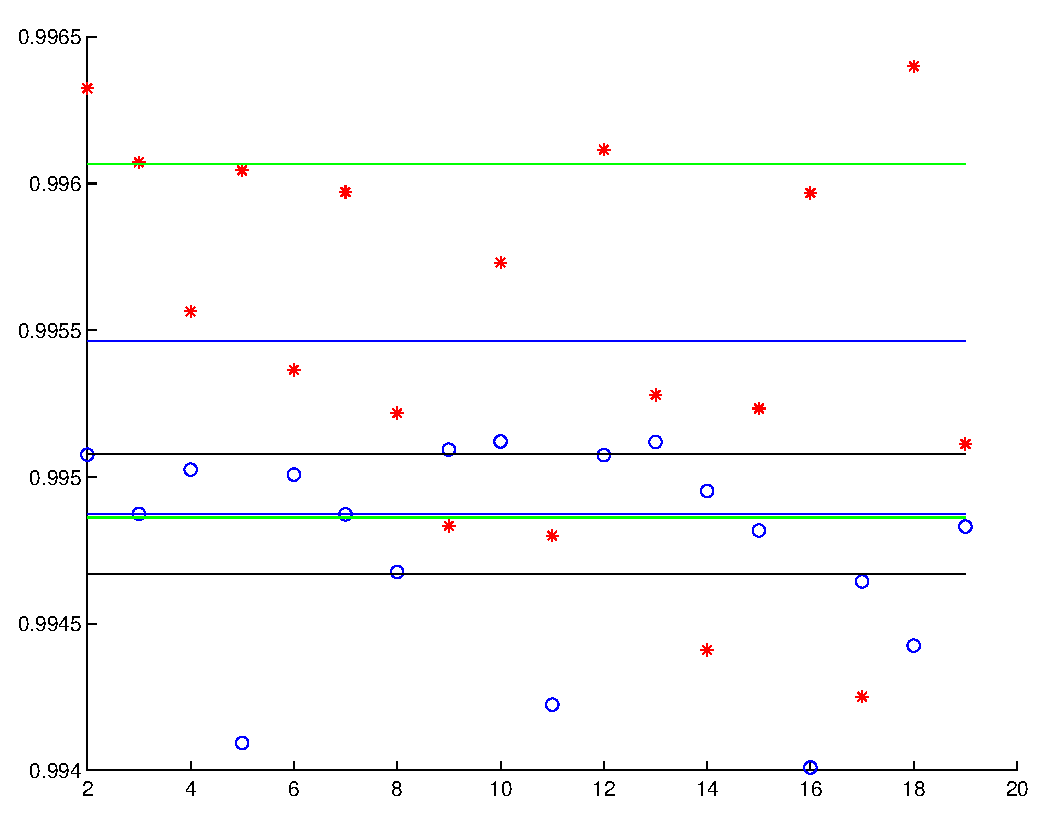
\includegraphics[width=1.00\linewidth]{Figures/fdllrep}
  \caption{The $18$ different settings for \bzip\ of the same setup}
  \label{fig:fdllrep}
\end{figure}

The blue lines in the figure show each median value for the geometric means, the green lines represent one standard deviation from the median for the \FDI\ case, while the black lines represent the standard deviation from the median for the \llvm\ case. As it can be seen, not only the values are too similar, varying only from the fourth decimal digit, but also the medians and their standard deviations overlap, collapse. This is a strong indicator that there is no significant difference between those measures.

So, what we did was to consider that a single-run experiment could have measured any of the strings individually, moreover, a single run may have also collected the best, or the worst values for the actual times of the experiment. Hence, to show a speedup for \FDI\, we collected the worst running time for \llvm\ inlined program, and the best running time for the \FDI\ inlined program. 

Even though the data showed a speedup, it was really worthless, only $0.46 \%$. Therefore, as we were not following the SPEC Benchmark suite, we made an "adjustment", we left the slowdowns and some of the tiny speedups gathered from the list of inputs outside the final list to be shown. This way we were able to present a tiny, but possibly measurable speedup, as in \refSection{sec:speedup}. To apply a list of inputs can be an issue, as this ``speedup'' shows, that is why a complete list of inputs containing all the explanations is a requirement when presenting data. The full data for the "speedup" experiment are shown in table \refTable{tab:fullexp}.

\begin{table}
  \centering
  \begin{tiny}
  
\begin{tabular}{lllll}

{\bf Input} & {\bf Normalized \FDO} & {\bf Normalized \llvm} & {\bf Speedup} \\ \hline

auriel & 0.9720 & 1.0076 & 0.9647   \\ 
avernum & 0.9922 & 0.9905 & 1.0017 \\
cards & 0.9909 & 0.9989 & 0.9919  \\
ebooks & 0.9909 & 0.9920 & 0.9988  \\
gcc & 0.9966 & 1.0059 & 0.9907  \\ 
lib-a & 0.9940 & 0.9970 & 0.9970  \\ 
mohicans & 1.0000 & 1.0048 & 0.9951  \\
ocal & 0.9988 &1.0075 & 0.9913  \\ 
paintings & 1.0000 & 1.0051 & 0.9949  \\
potemkin & 0.9916 & 0.9887 & 1.0029  \\
proteins-1 & 0.9977 & 0.9910 & 1.0068  \\
proteins-2 & 0.9813 & 0.9950 & 0.9862  \\
revelation & 0.9868 & 0.9887 & 0.9980  \\ 
sherlock & 1.0000 & 1.0020 &1.0125  \\ 
usrlib & 1.0000 & 0.9875& 1.0458  \\  \hline
Speedup & & & 0.9953 (0.46 \%) \\

\hline
\end{tabular}

  \end{tiny}
  \caption{Summary of the normalized data used to produce a speedup for \bzip}
  \label{tab:fullexp}
\end{table}

On the other hand, in \refSection{sec:slowdown} we did the opposite, we chose the worst individual running time for the \FDI\ inlined program and the best running time for the \llvm\ inlined program. Proceeding this way we showed that another individual measuring showed a slowdown. And as both results followed the same methodology, they are both correct, and this is unexplainable unless we consider that there is variance on the data.

We used the same process for the \gzip\ case using $20$ different settings, the \refFigure{fig:gzipfdll} shows the data collected in a similar way of \refFigure{fig:fdllrep}. In \refFigure{fig:gzipfdll} we can notice that there is actually a slowdown compared to \llvm\ for this setup, and even though we were able to report a speedup.

\begin{figure}
  \centering
  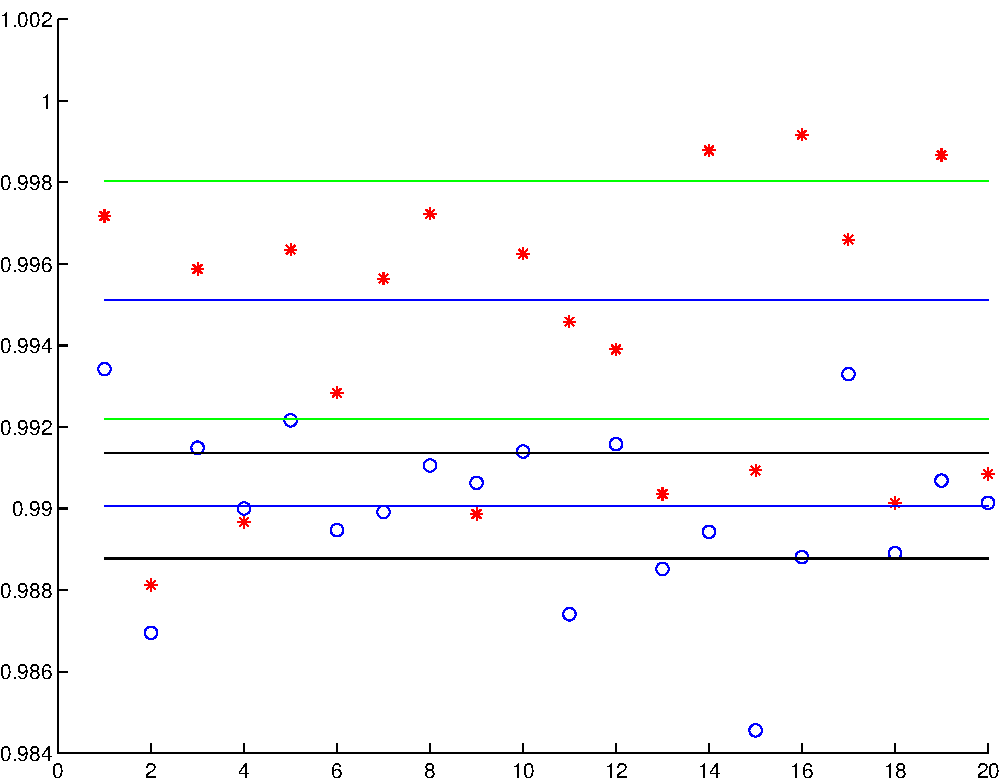
\includegraphics[width=1.00\linewidth]{Figures/gzipfdll}
  \caption{The $20$ different settings for \gzip\ of the same setup}
  \label{fig:gzipfdll}
\end{figure}

These cases were artificially constructed using our empirical actual data, considering that if we used a single-run methodology these results could appear. But as we were using \CP\ methodology, we were able to correctly identify that there is no statistical difference between both inliners, for the setup proposed. This result, in a certain way, reinforces the result of ~\cite{Curtsinger2013}, where they reported no speedup of $-O2$ over $-O3$ for all benchmarks they analyzed.

%=============== GCC

\subsubsection{Analysis of \gcc}

The same process was used for the \gcc\ case, we selected the best running times for the setting we had at each input, and from this we constructed our speedup experiment. In a single-run framework it is perfectly reasonable that this result can actually appear. But in this case we came up with a result considering a reduced input set, which produced an even better speedup. This was done to raise the question about the proper set of inputs to be employed. In fact, the set we presented in \refSection{sec:speedup} was already an extract from the SPEC CPU 2006 benchmark suite.

In reality we applied the full set and added 4 inputs, which were converted from the SPEC 2000 benchmark, \bzip, \lbm, \mcf, and \parser, fulfilling the 15-input set to each program. If we considered the full input-set we would have a different result, the speedup in the case of the best run-times, would be of $4.58 \%$, as shown in \refTable{tab:fullspeedup} and in \refFigure{fig:gccall}.

\begin{table}
  \centering
  \begin{tiny}
  
\begin{tabular}{lllll}

{\bf Input} & {\bf \FDO\ normalized} & {\bf \llvm\ normalized} & {\bf Speedup} \\ \hline

166 & 0.9494 & 0.9733 & 0.9754  \\
200 & 0.9617 & 0.9735 & 0.9879  \\
c-typeck & 0.9097 & 0.9745 & 0.9335  \\
cccp & 0.9650 & 0.9700 & 0.9948  \\
Cp-decl & 0.9554 & 0.9849 & 0.9700  \\
expr & 0.9035 & 0.9552 & 0.9458  \\
expr2 & 0.8630 & 0.9660 & 0.8934  \\
g23 & 0.9119 & 0.9849 & 0.9259  \\
integrate & 0.9811 & 1.0251 & 0.9570  \\
s04 & 0.9886 & 1.0181 & 0.9710  \\
scilab & 0.9945 & 1.0043 & 0.9902  \\
bzipR-all & 0.9870 & 1.0092 & 0.9780  \\
lbm-all & 0.8888 & 1.0000 & 0.8888  \\
mcf-all & 0.9487 & 1.0000 & 0.9487  \\
parser-all & 0.9945 & 1.0364 & 0.9596  \\
Geomean & & & 0.9541 \\
  
\hline
\end{tabular}

  \end{tiny}
  \caption{Summary of the normalized data used to produce a speedup for \gcc}
  \label{tab:fullspeedup}
\end{table}

\begin{figure}
  \centering
  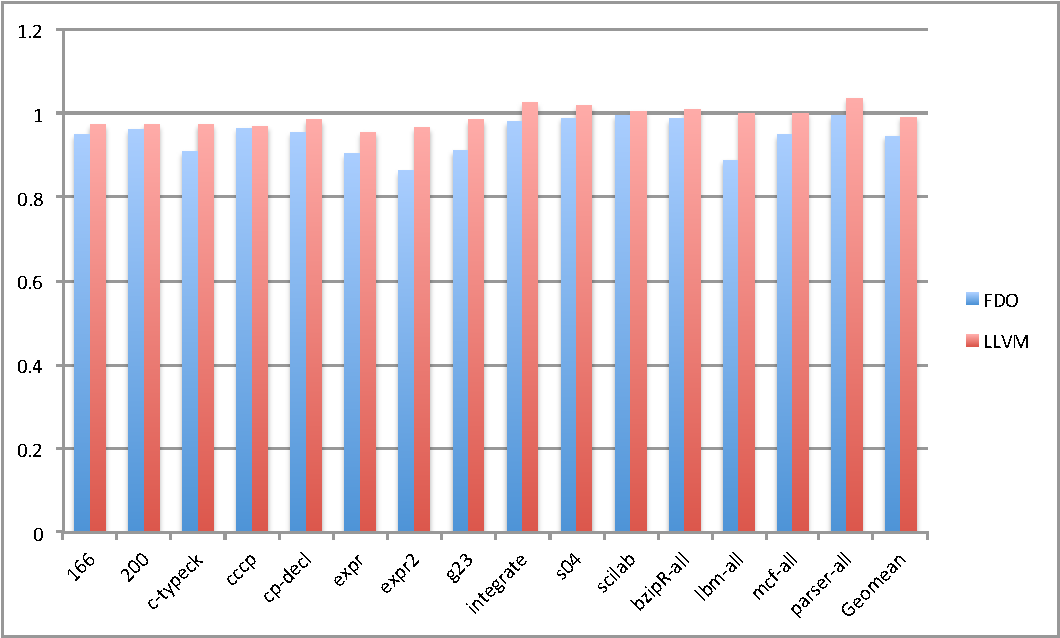
\includegraphics[width=1.00\linewidth]{Figures/speedupgccall}
  \caption{The $20$ different settings for \gcc\ of the same setup}
  \label{fig:gccall}
\end{figure}

Therefore, the input-set matters, as much as a sound methodology. To summarize this section we end this with a real outcome of our framework, where we can observe that there was not any speedups, or slowdowns for the case of \gcc, as can be easily seen from the error bars present in \refFigure{fig:gcc-results}. This figure is automatically generated by our system, and reflects the geometric mean of all inputs for twelve different \FDI\ inliners, the \llvm\ inliner (called static in the figure) and another static inliner called benefit.

\begin{figure}
  \centering
  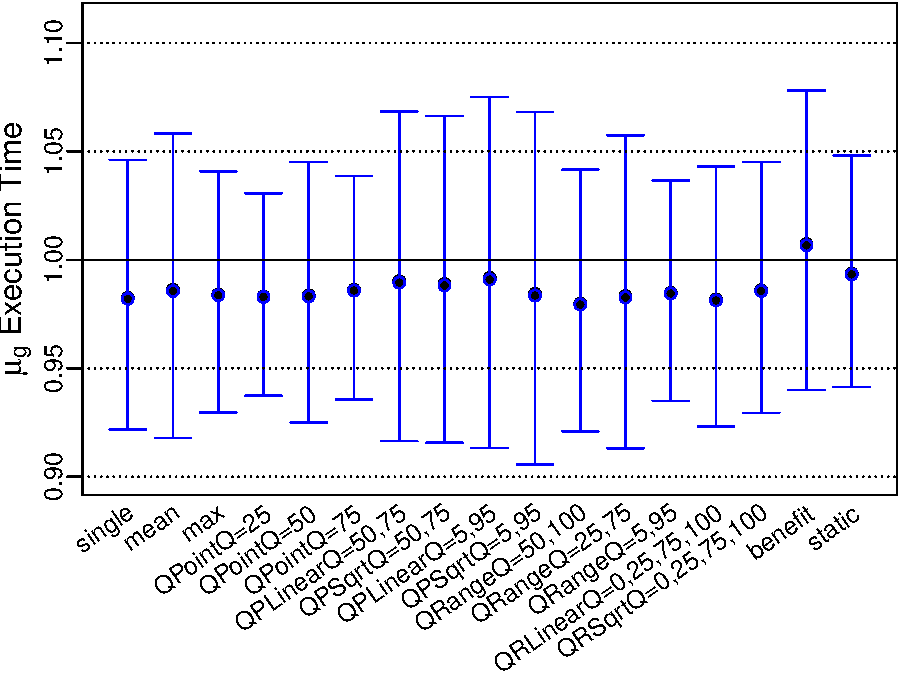
\includegraphics[width=1.00\linewidth]{Figures/gcc-results}
  \caption{The actual result for \gcc\ returned by our \CP\ framework}
  \label{fig:gcc-results}
\end{figure}

%============ regular text

In the next section (\refSection{sec:cmbprof}) we describe in more detail the \CP\ methodology, explaining its use and how we measure the results, in order to avoid the problems highlighted by the example in \refSection{sec:speedup}.
